% Astronomy data lake --- end-to-end pipeline flowchart.
% Companion to architecture_layers.tex (layered view).
%
% Compile to PDF (recommended for AASTeX / MNRAS):
%   pdftex -fmt=pdflatex pipeline_flowchart.tex
%
% Then in the paper:
%   \begin{figure*}
%     \centering
%     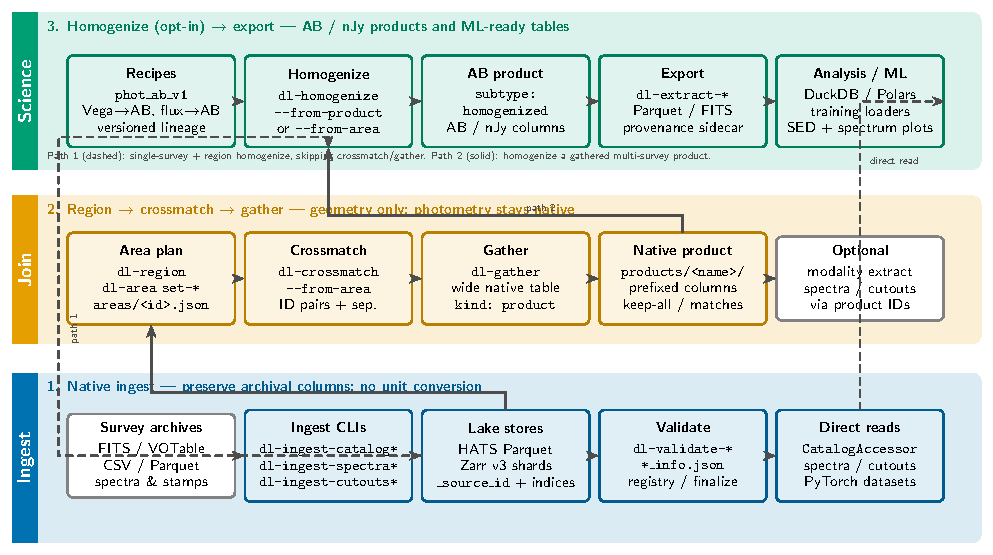
\includegraphics[width=\textwidth]{pipeline_flowchart}
%     \caption{End-to-end pipeline of the astronomy data lake.
%       Native survey archives are ingested onto HEALPix-tiled Parquet and
%       Zarr stores (blue). An area plan drives positional crossmatch and
%       gather into a wide native product (orange). Photometric
%       homogenization is opt-in (green), after which catalogs, spectra and
%       cutouts are exported for analysis and ML. Dashed arrows show
%       direct lake reads that skip the product path.}
%     \label{fig:lake-pipeline}
%   \end{figure*}
%
% Colour mapping (Okabe--Ito, print- and colourblind-safe):
%   blue   = foundation (native ingest / lake reads)
%   orange = area / crossmatch / gather
%   green  = homogenization + science export
%   grey   = external inputs / outputs

\documentclass[tikz,border=6pt]{standalone}

\usepackage{tikz}
\usetikzlibrary{arrows.meta,calc,fit,positioning,backgrounds}

\definecolor{oiBlue}{HTML}{0072B2}
\definecolor{oiOrange}{HTML}{E69F00}
\definecolor{oiGreen}{HTML}{009E73}
\definecolor{oiGrey}{HTML}{4D4D4D}

\begin{document}
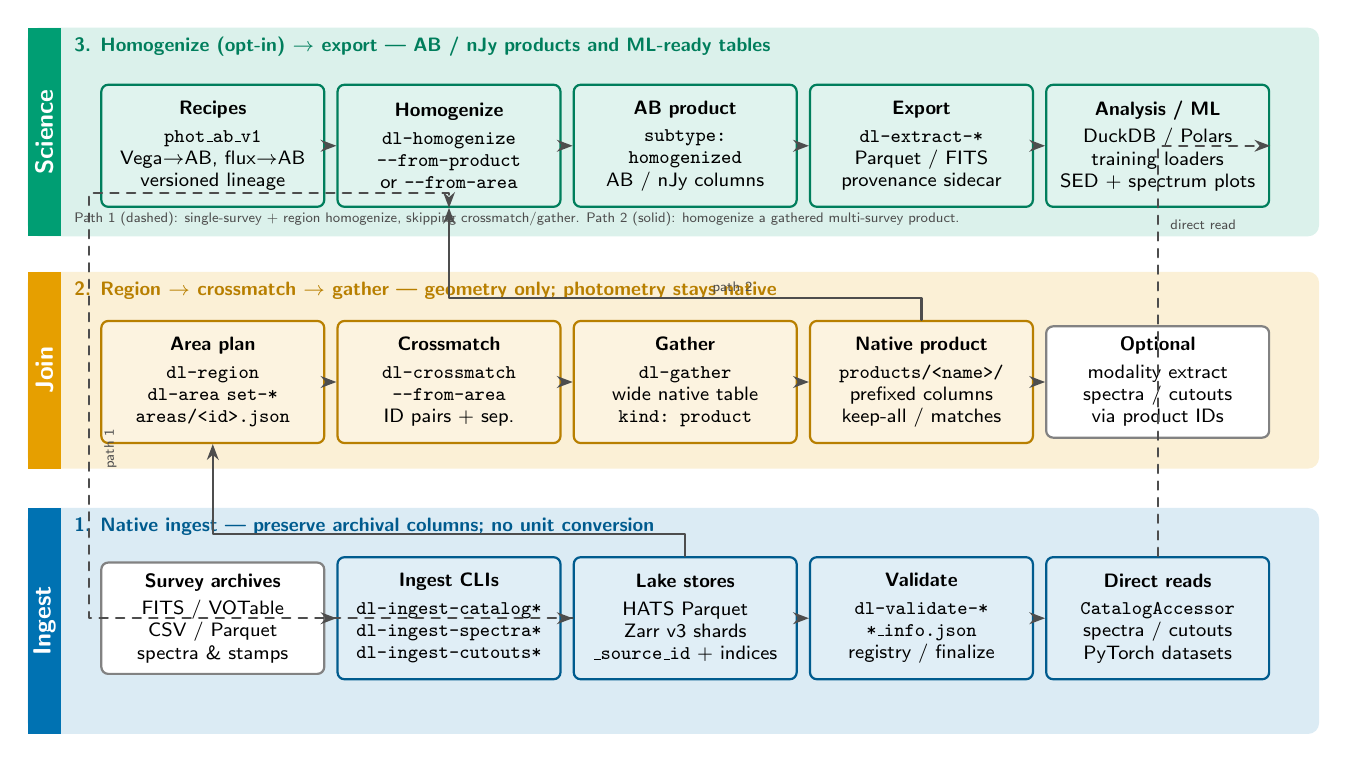
\begin{tikzpicture}[
  font=\sffamily\scriptsize,
  >=Stealth,
  line cap=round,
  line join=round,
  every node/.style={align=center},
  box/.style={
    draw=#1!80!black,
    fill=#1!12,
    thick,
    rounded corners=2.5pt,
    inner sep=4pt,
    text width=2.55cm,
    minimum height=1.55cm,
    font=\sffamily\scriptsize
  },
  extbox/.style={
    draw=oiGrey!70,
    fill=white,
    thick,
    rounded corners=2.5pt,
    inner sep=4pt,
    text width=2.55cm,
    minimum height=1.35cm,
    font=\sffamily\scriptsize
  },
  stage/.style={
    font=\sffamily\bfseries\scriptsize,
    text=#1!80!black,
    inner sep=1pt
  },
  bandlabel/.style={
    font=\sffamily\bfseries\small,
    rotate=90,
    anchor=center,
    text=white,
    inner sep=2pt
  },
  arr/.style={-{Stealth[length=2.0mm]}, thick, oiGrey},
  arrd/.style={-{Stealth[length=2.0mm]}, thick, dashed, oiGrey},
  note/.style={font=\sffamily\tiny, text=oiGrey, inner sep=1pt},
]

% Layout (cm)
\def\W{16.40}
\def\yIn{0.08}
\def\yInt{2.95}
\def\yJ{3.45}
\def\yJt{5.95}
\def\yS{6.40}
\def\ySt{9.05}
\def\cx{2.35}
\def\cA{5.35}
\def\cB{8.35}
\def\cC{11.35}
\def\cD{14.35}

\begin{scope}[on background layer]
  \fill[oiBlue!14, rounded corners=4pt] (0,\yIn) rectangle (\W,\yInt);
  \fill[oiOrange!16, rounded corners=4pt] (0,\yJ) rectangle (\W,\yJt);
  \fill[oiGreen!14, rounded corners=4pt] (0,\yS) rectangle (\W,\ySt);
  \fill[oiBlue] (0,\yIn) rectangle (0.42,\yInt);
  \fill[oiOrange] (0,\yJ) rectangle (0.42,\yJt);
  \fill[oiGreen] (0,\yS) rectangle (0.42,\ySt);
\end{scope}

\node[bandlabel] at (0.21,{0.5*(\yIn+\yInt)}) {Ingest};
\node[bandlabel] at (0.21,{0.5*(\yJ+\yJt)}) {Join};
\node[bandlabel] at (0.21,{0.5*(\yS+\ySt)}) {Science};

% ---------- Stage heads ----------
\node[stage=oiBlue, anchor=west] at (0.55,\yInt-0.24)
  {1. Native ingest --- preserve archival columns; no unit conversion};
\node[stage=oiOrange, anchor=west] at (0.55,\yJt-0.24)
  {2. Region $\rightarrow$ crossmatch $\rightarrow$ gather --- geometry only; photometry stays native};
\node[stage=oiGreen, anchor=west] at (0.55,\ySt-0.24)
  {3. Homogenize (opt-in) $\rightarrow$ export --- AB / nJy products and ML-ready tables};

% ---------- External input ----------
\node[extbox] (raw) at (\cx,1.55)
  {\textbf{Survey archives}\\[2pt]
   FITS / VOTable\\
   CSV / Parquet\\
   spectra \& stamps};

% ---------- Ingest CLIs / lake stores ----------
\node[box=oiBlue] (ing) at (\cA,1.55)
  {\textbf{Ingest CLIs}\\[2pt]
   \texttt{dl-ingest-catalog*}\\
   \texttt{dl-ingest-spectra*}\\
   \texttt{dl-ingest-cutouts*}};

\node[box=oiBlue] (lake) at (\cB,1.55)
  {\textbf{Lake stores}\\[2pt]
   HATS Parquet\\
   Zarr v3 shards\\
   \texttt{\_source\_id} + indices};

\node[box=oiBlue] (val) at (\cC,1.55)
  {\textbf{Validate}\\[2pt]
   \texttt{dl-validate-*}\\
   \texttt{*\_info.json}\\
   registry / finalize};

\node[box=oiBlue] (read) at (\cD,1.55)
  {\textbf{Direct reads}\\[2pt]
   \texttt{CatalogAccessor}\\
   spectra / cutouts\\
   PyTorch datasets};

% ---------- Join band ----------
\node[box=oiOrange] (area) at (\cx,4.55)
  {\textbf{Area plan}\\[2pt]
   \texttt{dl-region}\\
   \texttt{dl-area set-*}\\
   \texttt{areas/<id>.json}};

\node[box=oiOrange] (xm) at (\cA,4.55)
  {\textbf{Crossmatch}\\[2pt]
   \texttt{dl-crossmatch}\\
   \texttt{--from-area}\\
   ID pairs + sep.};

\node[box=oiOrange] (gath) at (\cB,4.55)
  {\textbf{Gather}\\[2pt]
   \texttt{dl-gather}\\
   wide native table\\
   \texttt{kind: product}};

\node[box=oiOrange] (nat) at (\cC,4.55)
  {\textbf{Native product}\\[2pt]
   \texttt{products/<name>/}\\
   prefixed columns\\
   keep-all / matches};

\node[extbox] (scratch) at (\cD,4.55)
  {\textbf{Optional}\\[2pt]
   modality extract\\
   spectra / cutouts\\
   via product IDs};

% ---------- Science band ----------
\node[box=oiGreen] (rec) at (\cx,7.55)
  {\textbf{Recipes}\\[2pt]
   \texttt{phot\_ab\_v1}\\
   Vega$\to$AB, flux$\to$AB\\
   versioned lineage};

\node[box=oiGreen] (hom) at (\cA,7.55)
  {\textbf{Homogenize}\\[2pt]
   \texttt{dl-homogenize}\\
   \texttt{--from-product}\\
   or \texttt{--from-area}};

\node[box=oiGreen] (ab) at (\cB,7.55)
  {\textbf{AB product}\\[2pt]
   \texttt{subtype:}\\
   \texttt{homogenized}\\
   AB / nJy columns};

\node[box=oiGreen] (exp) at (\cC,7.55)
  {\textbf{Export}\\[2pt]
   \texttt{dl-extract-*}\\
   Parquet / FITS\\
   provenance sidecar};

\node[box=oiGreen] (ml) at (\cD,7.55)
  {\textbf{Analysis / ML}\\[2pt]
   DuckDB / Polars\\
   training loaders\\
   SED + spectrum plots};

% Path-1 note under science band
\node[note, anchor=west] at (0.55,6.62)
  {Path~1 (dashed): single-survey + region homogenize, skipping crossmatch/gather.
   Path~2 (solid): homogenize a gathered multi-survey product.};

% ========== arrows ==========
% ingest row
\draw[arr] (raw) -- (ing);
\draw[arr] (ing) -- (lake);
\draw[arr] (lake) -- (val);
\draw[arr] (val) -- (read);

% foundation -> area (catalog sky selection)
\draw[arr] (lake.north) -- ++(0,0.28) -| (area.south);

% join row
\draw[arr] (area) -- (xm);
\draw[arr] (xm) -- (gath);
\draw[arr] (gath) -- (nat);
\draw[arr] (nat) -- (scratch);

% path 2: native product -> homogenize
\draw[arr] (nat.north) -- ++(0,0.28) -|
  node[pos=0.2, note, above] {path 2} (hom.south);

% science row
\draw[arr] (rec) -- (hom);
\draw[arr] (hom) -- (ab);
\draw[arr] (ab) -- (exp);
\draw[arr] (exp) -- (ml);

% path 1: lake -> homogenize via left gutter (skip join), matching
% architecture_layers.tex
\def\gutterx{0.78}
\draw[arrd] (lake.west) -- (\gutterx,1.55) -- (\gutterx,6.95)
  -- (hom.south |- 0,6.95) -- (hom.south);
\node[note, rotate=90, anchor=center] at (1.05,3.70) {path 1};

% direct reads also feed analysis (right rail)
\draw[arrd] (read.north) -- (\cD,6.15) -- (\cD,7.55) -- (ml.east);
\node[note, anchor=west] at (\cD+0.12,6.55) {direct read};

\end{tikzpicture}
\end{document}
